\documentclass{beamer}
\mode<presentation>
\usetheme{CambridgeUS}
\usepackage[russian]{babel}
\usepackage[utf8]{inputenc}
\usepackage[T2A]{fontenc}
\usepackage{sansmathaccent}

\usepackage{verbatim}
\usepackage{alltt}

\pdfmapfile{+sansmathaccent.map}
\title[Строки]{Строковый тип данных}
\author{Наумов Д.А., доц. каф. КТ, ИТГД }
\date[28.02.2020] {Программирование и алгоритмические языки, 2020}

\begin{document}

%ТИТУЛЬНЫЙ СЛАЙД
\begin{frame}
  \titlepage
\end{frame}
  
%СОДЕРЖАНИЕ ЛЕКЦИИ
\begin{frame}
  \frametitle{Содержание лекции}
  \tableofcontents  
\end{frame}
  
\section{Строковый тип данных}

\begin{frame}[fragile]
\begin{block}{Символ}
это буква, цифра или какой-либо знак. 
\end{block}
\begin{itemize}
\item Кодовая таблица символов ASCII состоит из 256 позиций; 
\item каждый символ имеет свой уникальный код от 0 до 255; 
\item один символ занимает 1 байт;
\item для работы с символами существует тип данных char.
\end{itemize}
\end{frame} 

\begin{frame}[fragile]
\begin{block}{Строка}
последовательность символов. 
\end{block}
В Lazarus строка трактуется как массив символов, то есть каждый символ строки пронумерован, начиная с единицы.

Константная строка (литерал строки) заключается в апострофы. 
\begin{alltt}
const S = 'СТРОКА';
\end{alltt}

Описание переменных строкового типа: 
\begin{alltt}
имя_переменной : string;
имя_переменной : string[длина_строки];
\end{alltt}
Если при описании строкового типа данных длина строки не указывается, это означает, что она составляет 255 символов. 
\end{frame}

\begin{frame}[fragile]
Присваивание строковой переменной константного значения: 
\begin{alltt}
s := 'Q';
s1 := 'Privet';
\end{alltt}
Объединение (конкатенация строк): 
\begin{alltt}
var s : string;
begin
s:= 'text_' + '_' + '*1' ;
(* Результат: строка 'text__*1' *)
\end{alltt}
\end{frame}  

\begin{frame}[fragile]
Доступ к отдельному символу: 
\begin{alltt}
var 
  s : string; 
  c : char;
begin
  s:= ’ Privet ’ ;
  c:= s[4] ;
(* Результат: c будет содержать значение 'v' *)
\end{alltt}
\end{frame}  

\begin{frame}[fragile]
\begin{alltt}
var
  Str1, Str2, Str3, Str4: String;
  word : String ;
  K, L : Integer ;
begin
  Str1:= 'Ivanov';
  Write('Enter string 2 -', Str1);
  ReadLn(Str2);
  Writeln('Str1: ', Str1);
  Writeln('Str2: ', Str2);
  //объединение 1-й и 2-й строк
  Str3 := Str1 + '_' + Str2;
  //определение длины строки
  L:= Length(Str3) ;
  Writeln('Str3: ', Str3) ;
  Writeln('Length of string 3 =', L);
\end{alltt}
\end{frame}

\begin{frame}[fragile]
\begin{alltt}
  Str4 := 'v';
  //поиск вхождения буквы v в строке 3
  K := Pos(Str4, Str3);
  Writeln('Fist accourance of v in Str3' ,K) ;
  //копирование в переменную Str4 6 символов, 
  //начиная с 8-го, из строки Str3
  Str4 :=copy(Str3, 8, 6);
  Writeln('Str4=', Str4) ;
  //поиск первого слова - копирование в переменную word 
  //символов из Str3, начиная с 1-го символа и до пробела
  Word := Copy(Str3, 1, Pos('_', Str3)-1);
  Writeln('First word is ' ,word) ;
  //удаление из Str3 двух символов, начиная с 5-й позиции
  Delete(Str3, 5, 2);
  Writeln('Result is ’, Str3) ;
  Readln;
end.
\end{alltt}
\end{frame}

%\begin{figure}
%\centering
%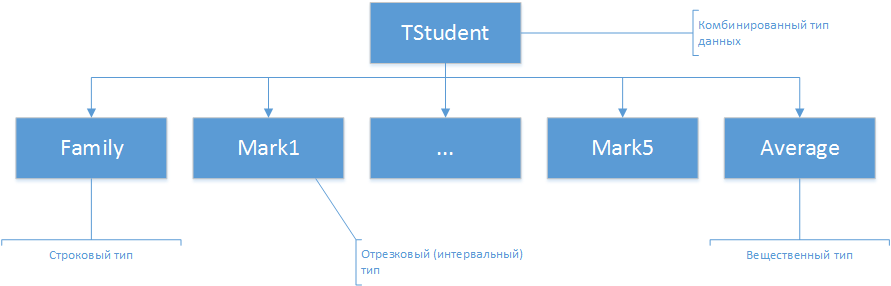
\includegraphics[scale=0.4]{images/record-01.png}
%\end{figure}


\end{document}
